\documentclass[
  msc,proposal,
  oneside,
  hidecover,
  hidededication,
  hideack,
  hideepigraph,
  hidelof,
  hidelot,
  hideabstract,
  hidecover,
  extraporttitlepagefalse
]{ppgccufmg}    

\usepackage[english]{babel}
\usepackage[latin1]{inputenc}
\usepackage[T1]{fontenc}
\usepackage{type1ec}
\usepackage{graphicx}
\usepackage{amsmath}
\usepackage{amsfonts}
\usepackage[a4paper,
  portuguese,
  bookmarks=true,
  bookmarksnumbered=true,
  linktocpage,
  colorlinks,
  citecolor=black,
  urlcolor=black,
  linkcolor=black,
  filecolor=black,
  ]{hyperref}
\usepackage[square]{natbib}
\DeclareMathOperator*{\argmax}{argmax}

\begin{document}

\ppgccufmg{
  title={Web data extraction in semi-structured documents},
  authorrev={de Freitas Veneroso, Jo�o Mateus},
  cutter={D1234p},
  cdu={519.6*82.10},
  university={Federal University of Minas Gerais},
  course={Computer Science},
  address={Belo Horizonte},
  date={2017-11},
  advisor={Berthier Ribeiro de Ara�jo Neto},
  approval={img/approvalsheet.eps}
}

% ==========================================
% Beginning of text.                       |
% ==========================================

\chapter{Introduction}

Web data extraction is the task of automatically extracting structured information
from unstructured or semi-structured web documents. It is a subset of the broader
field of Information Extraction, and thus it faces many of the same challenges. 

Structured information such as that found in a well organized relational database must 
conform to an underlying data model, namely an abstract model that formalizes
the entities and relationships in a given application domain. Unstructured information
however is not organized according to a logical model, therefore useful bits of data won't
be arranged cohesively and will ocasionally be permeated by chunks of irrelevant information.

Tipically, Information Extraction tasks consist of mapping unstructured or poorly
structured data to a semantically well defined structure. The input is usually
composed of a set of documents that describe a group of entities in a similar manner,
while the Information Extraction task deals with identifying those entities and 
organizing them according to a template. 

As an example, consider a collection of 
novels and the task of identifying the name of the main character in each novel. 
For this task, the model must first identify proper nouns and then understand the 
text sufficiently to allow inference on the relative importance of each noun. 

To achieve such a goal it is often useful to employ methods developed in the disciplines 
of Information Retrieval and Natural Language Processing. The former has achieved a 
great deal of success in the task of classifying documents according to statistical 
properties and the latter led to huge improvements in modelling human language.
Many times, the various methods employed in these disciplines lead to different 
approaches in the field of Information Extraction.

In the scope of this work, we are interested in the semi-structured data usually
found in HTML web documents. Web documents most often lie in between the 
structured-unstructured data paradigm, meaning that they take a rather
relaxed approach in regard to formal structure. Hierarchy, element disposition,
class names, and other features related to document structure and indirectly associated
with the data itself are valuable information in the task of identifying entities and 
determining relationships. So much that many times they are the major source of information 
for classification purposes, such as when extracting information from standardized tables.
However, far from a structured database, web documents usually provide very limited structure
to otherwise unstructured data such as that found in free text.

Our current focused research interest regarding web data extraction is collecting
computer science researcher information from university websites. We need this 
information in order to compare the reputations of national and international 
research groups in the area of computer science with the academic reputation ranking
metric proposed by \cite{Ribas2015} based on random walks over reputation graphs. 

It showed promising results when ranking publication venues and 
individual authors in the area of Computer Science by using information publically available in 
the DBLP repository (http://dblp.uni-trier.de/). However the DBLP database has sparse information 
about author affiliation and multiple records are outdated. To remedy this problem, in the past 
few years researchers from UFMG have been laboriously collecting this data manually, however
this process is tedious and inefficient. Currently, we only have affiliation information for 
about 1\% of the authors, being most of them from USA and Brazil and this is not nearly enough to 
allow broad international research group comparison.

Up to now, our goal has been to build an automatic information extraction system for
collecting author affiliation information from university websites. It has already 
achieved significant progress which shall be described further in section 3. However, the ideas 
developed in this concrete case will be further improved in order to construct a more general
approach to the broader Information Extraction task.

The research here described hopes to contribute by proposing a novel approach to the main 
Information Extraction task, making the computer science affiliation database available for 
further research and testing the quality of academic reputation metrics regarding 
research groups.

\chapter{Related Work}

In the last 20 years, the exponential growth of public information in the web has 
led to the development of a number of different approaches to the problem of web 
data extraction. Traditionally, the task was solved by designing special purpose
programs called wrappers to pinpoint relevant data and store it in some structured
format. The multiple tools varied wildly according to their degree of automation. 

It was readily perceived that manual wrapper generation was a rather tedious and
error prone process, unsuited for large scale operations. Already in 2000,
\cite{Kushmerick2000} advocated for wrapper induction, a technique for automatically
constructing wrappers. This approach is known in the literature by the acronym 
WIEN (Wrapper Induction ENvironment).

Web data extraction techniques often require some sort of assistance from human 
experts to boost accuracy. So the main challenge in the field lies in determining
an adequate tradeoff between degree of automation and precision.

In 2002, a survey by \cite{Laender2002} made a thorough classification of the
early approaches with a taxonomy based on their main technology, being them: languages for
wrapper development, HTML-aware tools, NLP-based tools, Wrapper Induction Tools,
Modeling-based tools and Ontology-based tools. Some noteworthy examples from this era
are: 

TSIMMIS \cite{Hammer1997} and WebOQL \cite{Arocena1999}, which are special purpose 
languages for building wrappers.

Road Runner \cite{Crescenzi2001}, XWRAP \cite{Liu2000} and W4F \cite{Sahuguet1999}, 
which are HTML-aware tools that infer meaningful patterns from the HTML structure.

RAPIER \cite{Califf1999}, SRV \cite{Freitag1998}, WHISK \cite{Soderland1999}, which 
are NLP-based tools.

WIEN \cite{Kushmeric2000}, Soft Mealy \cite{Hsu1998} and STALKER \cite{Muslea1999} which 
are wrapper induction methods.

NoDoSE \cite{Adelberg1998} and Debye \cite{Laender2002a}, which are semi supervised modeling
based tools that require some interaction with the user by means of a graphical
user interface.

In 2004, \cite{Flesca2004} developed a taxonomy emphasizing the advantages and 
drawbacks of web data extraction technologies according to the user viewpoint.
In 2006 \cite{Chang2006} complemented the previous surveys with new technologies.

In 2008 \cite{Sarawagi2008} classifies wrappers in the following three types: 
record-level, page-level and site-level wrappers. Record-level wrappers are only
able to process single records, page-level wrappers are capable of 
extracting data from a single page, and site-level wrappers are able to process
the whole webpage structure including subpages and their linking structure.

More recently, surveys by \cite{Ferrara2014} and \cite{Schulz2016} updated the 
previous surveys and included new approaches.

In 2016 \cite{Varlamov2016}, argued that the degree of automation can no
longer be the main classification criterion for the data extraction systems
because unsupervised methods which were widely considered to be the state 
of the art when dealing with individual websites performed poorly or were
innapropriate on cross site extraction tasks. The authors proposed a 
classification of methods by the extent of their application. 
The competing approaches were separated into two groups: methods for individual 
websites and methods that are applicable to whole application domains. 

The first group contains most of the earlier approaches, including the supervised
approaches: SRV \cite{Freitag1998}, RAPIER \cite{Califf1999}, WHISK \cite{Soderland1999}, 
WIEN \cite{Kushmeric2000} SoftMealy \cite{Hsu1998} and STALKER \cite{Muslea1999}; and
the unsupervised approaches: RoadRunner \cite{Crescenzi2001} and EXALG \cite{Arasu2003}.

The second group is divided between domain specific methods and domain agnostic methods.
Domain specific methods are designed for extracting data about a particular 
application domain across multiple websites. Our researcher name extractor 
method that will be further described on section 3 falls in this category. Domain
specific methods integrate information about the particular application domain in the 
course of its development and thus are able to achieve superior performance in
comparison to domain agnostic methods.

Domain agnostic methods are the most general extraction methods. They can extract
information from any application domain from multiple websites. They pose the hardest
challenge because the tool must infer data relevance without any prior training in
thar particular application domain. Some examples are: ODE \cite{Su2009}, ObjectRunner 
\cite{Abdessalem2010}, and AMBER \cite{Furche2012}. As previously stated,
these approaches tend to yield worse results than domain specific methods, however
recent research has been improving domain agnostic methods by large steps.


\chapter{Methodology}

This section describes briefly a statistical NLP approach to solve the researcher 
affiliation extraction problem presented in section 1. This problem is actually
composed of two parts. The first one envolves crawling university websites and
finding faculty repositories and the second one is extracting the actual researcher
affiliation data from these repositories. We will present here the model
developed up to now, and then we will present the further research goals that
are still to be reached.

\section{Crawler}

The crawling problem has been partially solved by online aggregators that
compiled university internet domains for most of the academic world. One of these
aggregators is https://univ.cc/, which contains links for the main websites of
9553 universities from 207 countries. These root domains were fed as seeds to
our crawler, that downloaded the entire websites and its subdomains, amounting
around 2 million documents. Once all webpages were downloaded the task at hand 
becomes identifying faculty repositories among the downloaded pages. 

This task can be accomplished quite efficiently by means of supervised machine
learning models once we have labeled a subset of the university webpages.
The labeling was manually done for 2440 pages, of which 373 were faculty repositories
and 2067 were other types of pages. We took care to select a proportional number
of pages from each country.

Since the classification task is not our main research focus, the results will
only be presented here briefly. Our classifier employed only 112 features:
\begin{itemize}
  \item 60 for the number of occurrences of a set of relevant keywords in the URL, the page 
         title, h1, h2 and h3 tags. Each element having its own set of features.
  \item 49 for the number of occurrences of a different set of keywords in the rest of the
        text of the page.
  \item 1 feature measuring the document length.
  \item 1 feature for the number of names found by a simplified version of the name extractor.
\end{itemize}

\begin{table}[h]
  \begin{center}
    \begin{tabular}{ |l|l|l| }
      \hline
      Model & Accuracy & Standard Deviation \\
      \hline
      Random Forest & 0.93 & 0.02 \\
      Gaussian Naive Bayes & 0.88 & 0.03 \\
      Linear SVM & 0.85 & 0.05 \\
      Logistic Regression & 0.90 & 0.02 \\
      \hline
    \end{tabular}
  \end{center}
  \caption{Classifier}
  \label{tab:classifier}
\end{table}

Four models were tested by means of 5 fold cross validation, the results are presented in
table \ref{tab:classifier}. All models except Support Vector Machines achieved a reasonable 
performance, however, since the Random Forest Classifier presented a more stable predictive 
capability, it was chosen as the classifier method for labeling the remaining webpages.

\section{Data extraction}

The data extraction stage consists of extracting researcher names from faculty directories.
The main challenge here is constructing a general enough approach that can be used 
effectively across different domains without extracting too much garbage together with the
valuable information. This task faces a typical precision vs. recall tradeoff.

\begin{figure}
  \centering
  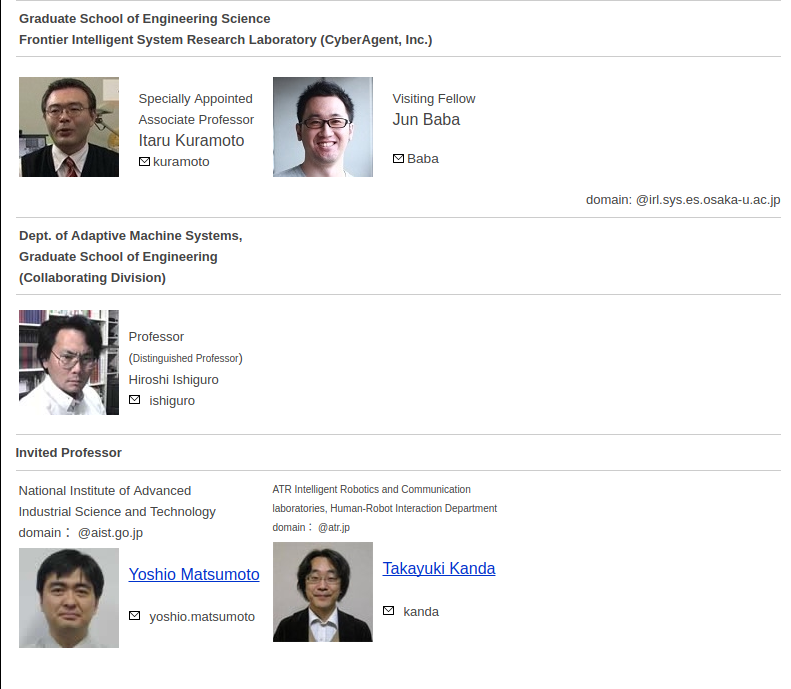
\includegraphics[width=1.0\textwidth]{pics/jap_intelligent_robotics_lab}
  \caption{Example of semi structured information}
\end{figure}

In order to understand the complexity of this extraction task take for example the
staff page for the intelligent robotics laboratory of Osaka University shown in figure 1.
Say we want to extract the name, position, email and picture of all members. It is easy to see
there is some sort of structure to the information we want to extract from this particular 
website, however, parts of the information are missing, repeated or disposed differently for
each particular member. If we want to go further it may be necessary to only extract information
from full members, a task that may pose a harder challenge. We may use grouping similarity 
combined with textual information in order to properly identify the desired entities.
In many cases the HTML element's relative position or CSS class name is sufficient to identify
particular occurrences of a same entity. If we do a good enough job at this first task we may 
extrapolate our model to extract information from similar web pages. 

However at this moment we are only interested in extracting researcher names and it is not
necessary to identify their status regarding full or partial membership.

\subsection{Proposed solution}

The name extraction problem is no different than a Named Entity Recognition problem, however 
approaches that tipically achieve a high accuracy on free text like Conditional Random Fields, 
Hidden Markov Models or Maximum Entropy Models perform very poorly in this particular case, 
because the data we are trying to extract is disposed in a tabular form and the words do not 
hold dependencies toward each other the same way they do in long pieces of text. In the name
extraction problem, structural HTML features and proper noun conditional probabilities play 
a key role.

Let $ t = (t_1, t_2, ..., t_n) $ be a sequence of tokens, and $ y = (y_1, y_2, ..., y_n) $ 
be a sequence of labels where $ y_i \in \{N, W\} \forall i \in \mathbb{N} $, such that $ y_i = N $ 
means token $ i $ is a name and $ y_i = W $ means token $ i $ is a word. The problem of extracting 
names from a sequence of tokens is equivalent to the problem of finding an optimal sequence of 
labels $ y^* $ for a sequence of tokens $ t $:

\begin{equation}
\\
y^* = \argmax_y P(t_i = y_i, t_{i+1} = y_{i+1}, ..., t_n = y_n)\\
\\
\label{eq:1}
\end{equation}

where $ P(t_i = y_i) $ is the probability that token $ t_i $ has label $ y_i $.
We may employ the chain rule to explore the relationship between the joint and conditional 
probabilities. Consider that $ P(Y_i) = P(t_i=y_i) $

\begin{equation}
\\
P(Y_1, Y_2, ..., Y_n) = P(Y_n) P(Y_2|Y_1) ... P(Y_n|Y_1, Y_2, ..., Y_{n-1})
\\
\label{eq:2}
\end{equation}

we could approximate these conditional probabilities the same way we would do for a
n-gram language model. However, the conditional probabilities $ P(t_i=y_i|t_{i-1}y_{i-1}, ...) $ are
hard to estimate because the joint disctribution $ P(t_i, y_i) $ depends both on the previous 
label and the previous token. If we express them in terms of joint probabilities the 
problem becomes clearer:

\begin{equation}
\\
P(t_i, y_i|t_{i-1}, y_{i-1}, t_{i-2}, y_{i-2}, ...)
\\
\label{eq:3}
\end{equation}

so we make the assumption that the probability that token $ t_i $ has label $ y_i $ depends
on the values of previous labels but is independent of the previous tokens. For example, 
given a sequence of tokens $ \{John, Hall\} $, the conditional probability $ P(Hall|John = name) $ 
is equivalent to $ P(Hall|any\ name) $. In other words, this means that the probability of 
Hall being a last name is the same regardless of a person's first name, as long as we can make sure 
that the previous token is a name. The conditional probabilities then become:

\begin{equation}
\\
P(t_i, y_i|t_{i-1}, y_{i-1}, t_{i-2}, y_{i-2}, ...) = P(t_i, y_i|y_{i-1}, y_{i-2}, ...)
\\
\label{eq:4}
\end{equation}

Replacing equation \ref{eq:4} in equation \ref{eq:2}, yields:

\begin{equation}
\\
P(Y_1, Y_2, \ldots, Y_n) = P(Y_1) P(Y_2|y_1) \ldots P(Y_n|y_1, y_2, ..., y_{n-1})
\\
\label{eq:4}
\end{equation}

We can once again employ the chain rule of probability to write:

\begin{equation}
\\
P(x_i, y_i|y_1, y_2, \ldots, y_{i-1}) = P(y_i|y_1, y_2, \ldots, y_{i-1})P(x_i|y_1, y_2, \ldots, y_i) \\
\\
\label{eq:5}
\end{equation}

Approximating $ P(x_i|y_1, y_2, ..., y_i) $ by $ P(x_i|y_i) $ we obtain:

\begin{equation}
\\
P(x_i, y_i|y_1, y_2, \ldots, y_{i-1}) = P(y_i|y_1, y_2, \ldots, y_{i-1})P(x_i|y_i) \\
\\
\label{eq:6}
\end{equation}

Take notice that $ P(Y_i) $ is a different notation for $ P(x_i = y_i) $ or $ P(x_i, y_i) $.
So, by replacing equation \ref{eq:6} in equation \ref{eq:4} we finally obtain:

\begin{equation}
\\
P(Y_1, Y_2, \ldots, Y_n) = P(y_1, y_2, \ldots, y_n) P(x_1|y_1)P(x_2|y_2) \ldots P(x_n|y_n) 
\label{eq:7}
\end{equation}

Equation \ref{eq:7} can be split into two parts: the prior, given by the first part of the 
equation on the right side and the conditional token probabilities, given by the rest of the 
equation on the right side. 

\subsubsection{Prior probabilities}

In order to obtain the prior probability, we need to acquire estimates for all possible 
sequences of labels. Considering that label $ y_i $ must be either a name or a word,
then there are $ 2^k $ different combinations for a window of size $ k $.

Let $ N $ be a name label and $ W $ be a word label, then for a window of size $ k $ we 
would need to estimate prior probabilities for all $ 2^k $ possible sequences of labels.
In practice, a window of size $ 4 $ seems to be accurate enough. In this case, the
sequences would be: $ \{W, W, W, W\}, \{W, W, W, N\}, \{W, W, N, W\}, \ldots $.

When names occur next to each other we have no way to tell where the first name ends and 
the second one starts. In order to delimit name boundaries we need to estimate
priors for different sequences of name labels in addition to our previous priors.
Let the first and second name labels be $ N_1 $ and $ N_2 $, respectively. Then,
we need to estimate priors for the sequences: $ \{W, N_1, N_1, N_2\}, 
\{W, N_1, N_1, N_2\}, \{W, N_1, N_2, N_2\}, \ldots $. In practice, we are never interested
in isolated occurrences of name labels so we can exclude combinations such as
$ \{W_1, N_1, N_2, N_2\} $.

Most of the times when names happen inside a list they tend to be contained inside a 
single HTML element. 
Eventhough this is not always the case, this knowledge can be incorporated as an
additional piece of evidence in our model. This evidence becomes specially useful 
when we are trying to delimit name boundaries. Let $ * $ indicate a breaking point in 
a sequence of labels, so $ {W, W*,N, N} $ means that the tokens taking labels WW
are contained inside a single HTML element, while the remaining tokens are inside 
different HTML elements.
We could estimate sequences with multiple breaking points, however a single breaking
point has shown good results. For our window of size 4, we need to estimate all prior 
probabilities with the 4 possible breaking points:
$ \{y_1, y_2, y_3, y_4\}, \{y_1*, y_2, y_3, y_4\}, \{y_1,y_2*, y_3, y_4\}, \{y_1, y_2, y_3*,y_4\}$.


\subsubsection{Conditional token probabilities}

We need to estimate conditional token probabilities for both labels: names and words.
So we need to know $ P(t_i|N) $, the probability that a name is $ t_i $ and
$ P(t_i|W) $, the probability that a word is $ t_i $.

For our experiments, the conditional token probabilities were obtained by maximum
likelihood estimation with Laplace smoothing to account for tokens that
didn't occur in the corpus. The $ P(t_i|N) $ probabilities were estimated over a 
collection of approximately 1.5 million names from the DBLP database. The
$ P(t_i|W) $ probabilities were estimated over a corpus of 100 thousand documents
obtained during the crawling stage. In the latter case all capitalized words 
were ignored when estimating probabilities in order to remove most names
from the corpus.

Token probabilities can be made more precise by incorporating features
in equation \ref{eq:7}. We do that by changing the token conditional 
probabilities to:

\begin{equation}
\\
P(t_i, f_1, f_2, \ldots, f_n|y_i) = P(t_i|y_i)P(f_1|y_i) \ldots P(f_n|y_i)
\\
\label{eq:8}
\end{equation}

where $ f_i $ are features, which are assumed to be independent between themselves.
The features can be textual or structural. Textual features take textual
clues like previous words and token length to predict if a given token is a name.
Structural features infer token probabilities based on the HTML structure
like tag names and nesting depth. In practice previous and 
next words weren't particularly effective in empirical tests, possibly due
to the fact that most names occured in lists in the test collection. So they were
removed from the features list.

Structural features estimated over the entire corpus end up being too general
so they help little in increasing token probability estimates. HTML structure 
varies radically between different documents such that the only stable characteristic 
is that names tend to have similar structural contexts in the same faculty
directory. For example, if all names appear inside a <tr> tag in a given document 
it does not mean that names tend to appear inside <tr> rather than any other tag
in other documents. However for that particular document we may be able to identify 
other names and exclude words by knowing that tokens occuring inside <tr> tags
have a higher probability of being names.

If our basic algorithm (without structural features) was able to extract a
good number of names from a page on the first passing, we may use
their structural context to estimate probabilities for our structural 
features. Of course those tokens that were tagged as words can be used
to estimate the word conditional probabilities. On a second passing we can
incorporate these improved estimates to boost the model's precision 
considerably. This process can be repeated multiple times to further 
increase peformance.

\begin{table}[h]
  \begin{center}
    \begin{tabular}{ |l|l|l| }
      \hline
      Id & Feature & Description \\
      \hline
      1  & Token incidence      & How often a token happens in a document's text  \\
      2  & Token length         & The token's character length                    \\
      3  & First+Second parents & First and second HTML parents combined          \\
      4  & Third parent         & Third HTML parent                               \\
      5  & CSS class name       & Innermost CSS class valid for the token         \\
      6  & Child number         & The child number in relation to the HTML parent \\
      7  & Nesting depth        & The number of HTML parents up to root           \\
      \hline
    \end{tabular}
  \end{center}
  \caption{Features}
  \label{tab:features}
\end{table}

Table \ref{tab:features} describes the features used in our experiments. A couple of
other features were tested, but they weren't included in our analysis because they didn't 
have a significant impact on the experimental results. Some of them are: next word
indicates some location (street, avenue, etc.), previous word is an honorific, 
token is capitalized, token is the first element in an HTML child, etc.


\subsection{Experiments}

\begin{table}[h]
  \begin{center}
    \begin{tabular}{ |l|l|l|l| }
      \hline
      Feature & Precision & Recall & F-measure \\
      \hline
      None  & 0.1 & 0.3 & 0.3 \\
      1     & 0.1 & 0.3 & 0.3 \\
      2     & 0.1 & 0.3 & 0.3 \\
      1+2   & 0.1 & 0.3 & 0.3 \\
      \hline
    \end{tabular}
  \end{center}
  \caption{Textual features experiment}
  \label{tab:base_model}
\end{table}

Experiments were made to determine the best model and the best set of features. The test collection 
was a set of 310 manually labeled faculty directory pages. For each model and each group of features 
the precision, recall and f-measure were calculated. Extracted names were only considered to be correct 
when they resulted on an exact match with the test data. All measures were obtained by the averaged 
results of a 5 fold cross validation run. We first compared the textual features on our base 
model (NE), which passes only one time over the token list. The results are presented on table 
\ref{tab:base_model}. 

\begin{table}[h]
  \begin{center}
    \begin{tabular}{ |l|l|l|l| }
      \hline
      Feature & Precision & Recall & F-measure \\
      \hline
      None  & 0.1 & 0.3 & 0.3 \\
      3     & 0.1 & 0.3 & 0.3 \\
      4     & 0.1 & 0.3 & 0.3 \\
      5     & 0.1 & 0.3 & 0.3 \\
      6     & 0.1 & 0.3 & 0.3 \\
      4     & 0.1 & 0.3 & 0.3 \\
      All   & 0.1 & 0.3 & 0.3 \\
      \hline
    \end{tabular}
  \end{center}
  \caption{Structural features experiment}
  \label{tab:ne_2}
\end{table}

Next, we tested the structural features in a model that passes two times over the 
token list (NE2) estimating the structural feature probabilities on the second passing. 
We used the best set of textual features found in the previous experiment. The results 
are presented on table \ref{tab:ne_2}.

\begin{table}[h]
  \begin{center}
    \begin{tabular}{ |l|l|l|l| }
      \hline
      Number of passings & Precision & Recall & F-measure \\
      \hline
      1   & 0.1 & 0.3 & 0.3 \\
      2   & 0.1 & 0.3 & 0.3 \\
      3   & 0.1 & 0.3 & 0.3 \\
      4   & 0.1 & 0.3 & 0.3 \\
      5   & 0.1 & 0.3 & 0.3 \\
      \hline
    \end{tabular}
  \end{center}
  \caption{Multiple passings experiment}
  \label{tab:ne_plus}
\end{table}

Finally we compared models with 1, 2, 3, 4 and 5 passings over the token list using the 
best set of features from the previous experiments. The results are presented on 
table \ref{tab:ne_plus}.


\subsection{Further Research}

Our model is finely tuned for the particular problem of researcher name extraction, 
but we believe this result can be generalized to solve other data extraction 
problems. Furthermore, the researcher affiliation data collected by the name extractor 
still needs to be used for evaluating the reputation metric proposed by \cite{Ribas2015}
in the research group classification task.

\chapter{Schedule}

The dissertation project will be divided into 6 tasks that shall be accomplished
along 2018. The tasks are:

\begin{enumerate}
  \item \textbf{Literature review}: review the literature about the topic of research
  \item \textbf{Data analysis}: collect and structure the relevant data.
  \item \textbf{Baseline}: recreate some key approaches from the literature.
  \item \textbf{Model implementation}: implement the general approach of the model described in section 3.
  \item \textbf{Experiments}: compare the implemented model with the baseline.
  \item \textbf{Dissertation}: write the dissertation and reviewing the text.
\end{enumerate}

\begin{table}[h]
  \begin{center}
    \begin{tabular}{ |c|c|c|c|c|c|c|c|c|c|c|c|c| }
      \hline
      Task & Jan & Feb & Mar & Apr & May & Jun & Jul & Aug & Sep & Oct & Nov & Dec \\
      \hline
      \hline
      1 & x & x & x &   &   &   &   &   &   &   &   &   \\
      \hline
      2 & x & x & x &   &   &   &   &   &   &   &   &   \\
      \hline
      3 &   &   &   & x & x & x &   &   &   &   &   &   \\
      \hline
      4 &   &   &   & x & x & x &   &   &   &   &   &   \\
      \hline
      5 &   &   &   &   &   &   & x & x & x &   &   &   \\
      \hline
      6 &   &   &   &   &   &   & x & x & x & x & x & x \\
      \hline
    \end{tabular}
  \end{center}
  \caption{Schedule 2018}
  \label{tab:schedule}
\end{table}


% ==========================================
% End of text.                             |
% ==========================================

\ppgccbibliography{bibfile}
\nocite{*}

\end{document}
